\documentclass[12pt]{article}

\usepackage{fullpage}
\usepackage{graphicx, rotating, booktabs} 
\usepackage{times} 
\usepackage{natbib} 
\usepackage{indentfirst} 
\usepackage{setspace}
\usepackage{grffile} 
\usepackage{hyperref}
\usepackage{adjustbox}
\setcitestyle{aysep{}}


\singlespace
\title{\textbf{Summary of Previous Empirical Work on the Arms-Alliances Tradeoff}}
\author{Joshua Alley\footnote{Graduate Student,
Department of Political Science, Texas A\&M University.}}
\date{{\normalsize \today}}

\bibliographystyle{apsr}

\begin{document}

\maketitle 


\section*{Introduction}

Military spending and alliance behavior the two of best-studied security policies in international relations. Despite the individual salience of arms spending and alliances, we know much less about how these policies impact one another. This shortcoming is the result of limitations in theory and research design. Although current scholarship has defects, those defects can be overcome, and it also provides material to build on.    

States can use their own or allied military resources as a source of capability. Because military spending and allies provide military capability, scholars believe these two policies affect one another, creating an arms-alliances tradeoff. To assess research on this tradeoff, I undertook a comprehensive review of scholarship on the association between alliance behavior and domestic defense effort. The review cataloged the primary claim, theory, research design, and evidence of 27 papers.\footnote{In the interest of parsimony, I did not comprehensively address free-riding in NATO. Instead, I focused on work in that literature made a major methodological or theoretical contribution.} 
 
Theory on the arms-alliances tradeoff has made some valuable inroads during a debate over whether alliance membership increases or decreases military spending. There are two competing perspectives--- one sees arms and allies as substitutes, while the other argues that these policies are complements. Neither perspective incorporates the key insights of the other, which has stunted theoretical progress. Substitution theory omits foreign policy goals besides security, while complementarity theories ignore domestic political incentives to limit military spending. 

Serious empirical flaws in many studies have constrained our ability to assess the relative merits of complementarity and substitution theories. Many scholars test their claims with limited samples and misspecified models. Evidence from a few reliable studies suggests that the association between alliance membership and military spending may be conditional. 

Although the relationship between arms and alliances has multiple components, most inquiry has focused on how alliance membership affects military spending. In turn, most work on alliance membership and military spending addresses the prevalence of free-riding. The emphasis on free-riding created serious research design problems, and left several other research questions in the arms-alliances tradeoff unanswered. We have no theory on how the international context affects the arms-alliances tradeoff, and no general evidence of how the costs of alliance formation affect domestic military spending. Addressing these and other research questions will sharpen understanding of the arms-alliances tradeoff, as well as the relative merits of complementarity and substitution theories. 

Clarifying the relationship between arms and alliances is important. The common perception that alliances lead to reduced defense spending guides policy, as US policymakers attempt to redress perceived opportunism. But inasmuch as free-riding is a poor explanation of the arms-alliances tradeoff, it is unlikely to inform effective policy. 

This paper summarizes prior scholarship and suggests some directions for future inquiry. I start by examining the theoretical logic behind theories of arms and allies as substitutes and complements. Then I assess the validity of prior research design and empirical evidence. The last section concludes by discussing open issues in the arms-alliances tradeoff literature and considerations for future research. 


\section*{Arms and Allies as Substitutes}

If arms and alliances are substitutes, then additional alliances or capability from alliance partners should lead to decreased domestic military spending.\footnote{Most empirical tests focus on this prediction, although substitution logic also predicts that when alliances become more costly, states will turn to domestic arms.} Two distinct theories predict this inverse association between alliance membership and domestic arms. Substitution theories of the arms-alliances tradeoff and the economic theory of alliances focus on how arms and allies both produce security, leading states to replace domestic military spending with allied spending. 

Both approaches motivate substitution through the opportunity costs of military spending. Although military spending can have positive economic and technological spinoffs \citep{DegerSen1995, WhittenWilliams2011}, allocating funds to the military takes resources away from other social and economic policies. Leaders can use these public and private goods to ensure their survival in office \citep{BDMetal2002}. Therefore if states have ample domestic political motives to reduce spending and rely on their allies to provide security. 

Predictions of substitution between arms and alliances rely on the insight that states can use multiple policies means to achieve their foreign policy goals \citep{MostStarr1989}. \citet{Morrow1993} argues that domestic arms and alliances are both sources of military capability, allowing states to substitute between the two in their search for security. Instead of internal balancing through spending more on domestic arms, states can rely on external balancing through allied capability \citep{Conybeare1992}. 

The marginal costs of arms and alliances determine which policy states use to increase their security \citep{Sorokin1994}. For instance, some evidence suggests that as the opportunity cost of military spending increases, states are more likely to form alliances \citep{Kimball2010, AllenDigiuseppe2013}. Measuring the foreign policy costs of a potential alliance is the main barrier to examining whether higher costs of an alliance lead states to rely more on military spending. Because the costs of arms are financial, while the costs of alliances are measured in foreign policy freedom, arms and alliances are not perfect replacements. 

As a source of capability, arms and allies are imperfect substitutes. States can rely on their own arms in any contingency, but domestic military capabilities take a long time to develop. Because members have divergent foreign policy interests, alliances are a less reliable source of capability than domestic arms, but provide immediate capability gains. The moment a treaty enters into force, alliance members gain their partner's support.

More reliable alliances are more like domestic arms as a source of capability. Therefore, credible alliance treaties are a better substitute for domestic arms. \citet{DigiuseppePoast2016} expand on this insight by arguing that because defense pacts with a democracy are more credible, these alliances will lead to reductions in spending. 

The theoretical logic of substitution theory is clear, but we have little evidence for these claims. Only four studies test substitution of alliances for arms using military spending or personnel as the dependent variable. This lack of attention is due to the provocative claim that alliances lead to free riding, which has received more attention. 

\subsection*{Free Riding and the Economic Theory of Alliances} 

The economic theory of alliances predicts that alliances lead to reduced domestic arms spending, but relies on a different mechanism. \citet{OlsonZeckhauser1966} treat security from an alliance as a public good, which generates a collective action problem for members. Each member's military spending is a contribution to the public good, but all members have incentives to free ride on their partners' expenditures. As a result, they predict that larger members of an alliance will bear a higher defense burden, because these states have a higher absolute value of the public good. Olson and Zeckhauser interpret a positive correlation between GDP and the ratio of defense spending to GDP as evidence of free-riding. Under this theory, alliance membership leads smaller states to reduce defense effort. 

Olson and Zeckhauser's claims sparked extensive debate about free riding by alliance members. Much of the discussion focused on NATO, but other scholars checked the correlation between defense burdens and GDP in other alliances, with mixed results \citep{Reisinger1983, Thies1987, GatesTerasawa1992, OnealWhatley1996, Siroky2012}. The best evidence of free-riding is work by \citet{PluemperNeumayer2015}, who show that many NATO allies are unresponsive or even reduce spending when growth in Soviet spending exceeds growth in US spending, and that the degree of free-riding depends on distance from the USSR. As with substitution theories, free-riding may only occur when treaty commitments are sufficiently credible \citep{GatesTerasawa1992}. 

A theoretical extension of the economic theory of alliances relaxes the public goods treatment of military spending. The joint product model treats military spending as having public and private benefits \citep{ConybeareSandler1990}, which lead to different predictions. As the ratio of private to public benefits from military spending increases, we should observe less free-riding \citep{Murdoch1995, SandlerHartley2001}. Differentiating between public and private benefits is difficult, however. Some studies divided types of military spending according to the benefit they provide, especially nuclear and non-nuclear defense effort \citep{Hansenetal1990}. Nuclear arms provide a pure public good through deterrence, while conventional spending has private benefits such as increased border security. 

Emphasizing free riding creates theoretical and empirical issues. The concept of free-riding itself is problematic. Reductions in spending by NATO members could reflect decreased threat perceptions or a bargain with the United States \citep{Lanoszka2015}. Distinguishing between free-riding and exchange is difficult, especially if smaller alliance members trade security for autonomy in asymmetric alliances \citep{Morrow1991}. 

The focus on burden sharing in the economic theory of alliances then leads to research design problems complications. The standard indicator of free riding is a state's defense burden--- military spending as a share of GDP. It is difficult to identify a model of this ratio variable, especially with GDP on both sides of the equation, casting serious doubt on many of the studies that rely on correlations between defense burdens and economic size as evidence \citep{PluemperNeumayer2015}. 

Despite problems from the focus on free-riding in the economic theory of alliances, substitution theories of alliances have a clear internal logic and mechanism. Because of this clarity, substitution theory is the best known theoretical paradigm in the arms-alliances tradeoff literature. Policymakers complaints about free-riding further reinforced the perception that alliances lead to reduced defense effort. 

The major weakness of substitution theories is their emphasis on security as the only output of an alliance. Substitution theory acknowledges that multiple policies can advance a state's security, but it does not incorporate other foreign policy goals, such as autonomy. Therefore, this perspective cannot capture the full range of how alliances may affect domestic arms. 

States have a range of foreign policy goals. Even security focused paradigms like neorealism admit states may have different preferences over whether to maintain or change the status quo \citep{Schweller1994, Walt2009}. Substitution theory addresses some of the domestic political incentives states face in making security policy, but it provides little detail about possible differences in foreign policy. By contrast, theories of arms and alliances as complements include diverse foreign policy aims. 


\section*{Arms and Allies as Complements}

The literature on arms and alliances as complements is less well developed. These theories expect that arms and alliances are positively correlated--- alliance membership leads to increased military spending. There are several tentative explanations for this prediction.

\citet{Diehl1994} argues that arms and alliances are not comparable policies and have multiple purposes besides deterrence, so substitution is unlikely. He then lists several possible mechanisms behind complementarity between arms and alliances, but does not articulate which is most important. These mechanisms include the possibility that alliances require increased foreign policy activity, or that major powers increase military spending to cover free-riding by junior alliance partners. The most general argument asserts that autonomy benefits from an alliance increase the marginal value of military spending, which is the main argument of complementarity theories. 

\citet{MorganPalmer2006} also use an increase in the marginal benefit of military spending to explain complementarity between arms and alliances. Their theory starts with the premise that states have two foreign policy goals--- maintenance and change. States then allocate all their foreign policy resources to pursue a mix of maintenance and change across a range of issues. Due to budget constraints, there is a tradeoff between maintenance and change. Within this framework, Morgan and Palmer examine substitution between policies by starting with the assumption that states choose the most efficient policy tool to realize their goals. 

Given the efficiency assumption, there are three reasons states might increase their use of a particular policy. The first is an increase the overall resources available to the state, and the second is changes in relative preferences for maintenance and change. The last path is changes in the efficiency of different policies, which is the only path that leads to substitution. In this model, substitution is motivated by states moving resources from less to more efficient policies, which they claim is uncommon. 

Rather, Morgan and Palmer argue that alliances increase the amount of resources available to the state, which frees up additional resources to pursue other goals. Alliances expand the foreign policy possibilities for a state, which makes them more likely to increase military spending. As an illustrative example, they argue that an alliance with the US gave Britain and France extra resources to pursue change in the Middle East during the 1957 Suez crisis.  

Because states do not expend the same kinds of resources on domestic arms and alliances, the concept of a foreign policy ``budget'' is nebulous, and it does not incorporate domestic policy at all. Neither Diehl nor Morgan and Palmer adequately explain the process by which joining an alliance increases military spending. Greater clarity about the mechanism by which alliances increase the marginal benefits of military spending is necessary. Otherwise, we are left with theories that have minimal process, and merely assert that arms and alliances have complementary characteristics. 

A different complementarity mechanism is cooperation and policy coordination between alliance members. The cooperation thesis acknowledges collective action problems among alliance members, but asserts that these problems can be overcome. \citet{Palmer1990} conceptualizes relations among alliance members as an iterated prisoner's dilemma, where states can communicate and use side issues to overcome collective action problems. \citet{QuirozFlores2011} attributes a positive spatial correlation in the defense burden of allied states to increased cooperation between allies. 

There is evidence that alliances facilitate cooperation in other issue areas \citep{Gowa1995, GowaMansfield2004, Poast2012, Poast2013}. But payments on side issues will not necessarily lead to increases in spending. Small states can use concessions on other issues as part of a bargain with their patron that allows for reduced military spending--- this is the same kind of exchange that makes the concept of free-riding problematic. Intra-alliance cooperation is an insufficient explanation of complementarity between arms and allies because it avoids dealing with exchange and elides domestic political incentives to reduce defense spending. 

The challenge for complementarity theory is clear--- scholars must develop better theoretical explanations for their prediction that alliance membership leads to increases in military spending. The shortcomings of current theories do not imply that scholars should rule out complementarity between arms and alliances, however. Theories of arms and allies as complements still make a valuable contribution to knowledge of the arms alliances tradeoff by considering diverse foreign policy goals.

\section*{The State of Arms-Allies Theory}

Given arguments that arms and alliances are complements or substitutes, what is the overall theoretical development of the literature? The two perspectives have distinct strengths and weaknesses, but debate over whether arms and allies are substitutes or complements treats the two perspectives as incompatible. Framing substitutes and complements as competing hypotheses has stunted theoretical progress, as neither perspective incorporates the key insight of the other. 

Substitution theory has not engaged with the claim that states have diverse foreign policy goals. Complementarity theories ignore domestic political incentives for security-seeking states to rely on allied capability. Because the strengths and weaknesses of these perspectives mirror each other, it may be possible to combine the two. Rather than pitting complementarity and substitution theories against each other, a general approach should consider whether each applies in different circumstances. This combination implies a conditional association between arms and alliances. 

\citet{DigiuseppePoast2016}'s theory is a useful first step towards a conditional theory. They argue that states will only reduce substitute alliances for arms if the alliance is sufficiently credible, and that democracies make more credible alliance promises. By acknowledging heterogeneous effects of alliances, their theory and results suggest that arms and alliances are not uniformly substitutes or complements. 

Regardless of how theories of the arms-allies tradeoff evolve, they must offer more precise hypotheses. Many theories do not specify clear observable implications of an arms-alliances tradeoff, beyond some advice to focus on marginal changes \citep{Morrow2000, Starr2000}. Others are less clear about the scope conditions of their theories. Without precise theoretical predictions, the risk of spurious results from poor research designs increases. 

The debate over free-riding in alliances is an example of the research design problems that result from inadequate attention to scope conditions. Most scholars ignore possible differences between major and non-major powers. The economic theory of alliances expects greater free riding by smaller alliance members, but many tests of this theory examine alliances between major powers \citep{Thies1987, ConybeareSandler1990, Siroky2012}, which may not have large enough size differences.  

The scope conditions problem points to another major challenge in scholarship on the arms-alliances tradeoff--- many empirical results have limited viability. Absent reliable empirical results, assessing the relative value of different theories is impossible. Despite the general claims in different theories, most studies of the arms-allies tradeoff provide poor evidence for their claims. Many researchers use limited samples of states or alliances, or fail to account for critical empirical problems.   





\section*{Empirical Challenges}

Estimating the association between arms and alliances is difficult. The following section summarizes research design in studies of the arms-allies tradeoff, and whether these studies addressed key problems. Any research design must consider causes of simultaneous change in arms and allies, measurement, and scope conditions. Besides these theoretical aspects of research design, military spending is a challenging dependent variable. National military spending is highly autocorrelated, and its skewed distribution is problematic for conventional regression estimators. 

Few studies estimate the general association between alliances membership and arms. Only six researchers use military expenditures as the dependent variable, and account for the presence of multiple alliances. Five of these six models are untrustworthy, as they do not control for key correlates of spending and use limited samples. 

For example, \citet{MorganPalmer2003} regress changes in military expenditure on indicators of state and alliance capabilities. Their sample is the year after a state's alliance portfolio changed, and the model includes no control variables, raising the risk of selection and omitted variable bias. Other studies focus only on great power alliances \citep{ConybeareSandler1990, Conybeare1994, Diehl1994, MostSiverson1987}, with little attention to possible differences in how these states make defense allocations. While great powers face salient security threats, a better empirical approach is to control for differences in threat. 

Eighteen other studies examine dynamics within specific alliances. These research designs address alliance-level variation in more detail, looking at specific changes in the political context or nature of the alliance itself. Seven of these studies examine NATO or the Warsaw Pact only. Much of the work on specific alliances tests whether larger members have a higher defense burden, in accordance with the primary prediction of the economic theory of alliances. Early studies of free-riding in specific alliances rely on correlation coefficients or regressions with 20 or fewer observations \citep{OlsonZeckhauser1966, Starr1974, Reisinger1983, Siroky2012}, where there is a high risk of spurious results. 

The focus on specific alliances is driven by data availability--- NATO members and great powers have more data on military spending. Even so, some focused studies provide plausible estimates. \citet{PluemperNeumayer2015}'s quasi-spatial model of how NATO members respond to US and Soviet spending is the best evidence of free-riding by NATO members. \citet{Sorokin1994} takes a similar approach to estimating the responses of four states to the military spending of a key ally with a two-stage least squares GLS estimator.

Most studies, whether specific or general, ignore autocorrelation in the data-generating process of military spending. Past military spending is an excellent predictor of future spending. Therefore time-series observations within states are not independent, but many studies treat these observations as independent. Four of the 26 studies use an estimator or specification that incorporates autocorrelation in military spending. Four others use a differenced dependent variable. 

Even when accounting autocorrelation, the standard linear regression estimator may be inefficient. When the regression residuals are not normally distributed, OLS is still unbiased, but it is not the minimum variance estimator \citep{RaineyBaissa2017}. As \autoref{fig:milex_histogram} shows, military spending from 1950-2001 is not normally distributed, even after applying a log transformation. As a result, regression models that use this data will likely have skewed residuals as well, making their estimates inefficient. 

\begin{figure}
	\centering
		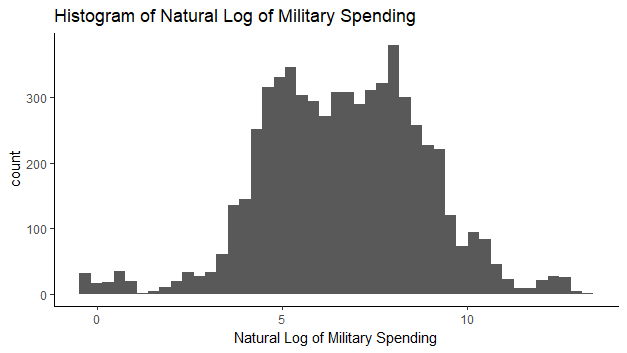
\includegraphics[width=0.95\textwidth]{milex_histogram.png}
	\caption{Distribution of Annual Military Spending by all States: 1950-2001}
	\label{fig:milex_histogram}
\end{figure}

Given all of these concerns, the best model of the arms alliances tradeoff is the work of \citet{DigiuseppePoast2016}, who find that substitution of alliances for arms is conditional on the credibility of the alliance. They argue that that democracies make more credible commitments, and estimate regression models of the association between defense pacts with a democracy and the natural log of military spending, using a lagged dependent variable to account for autocorrelation. This research design is a marked improvement over prior tests of how alliances affect domestic military spending.\footnote{While their regression estimator does not account for heavy tails in the dependent variable, the results are robust to using a robust regression estimator.} 
 

\subsection*{Arms Costs and Alliance Formation}

Only two studies consider the another facet of the arms-alliances tradeoff--- how the opportunity costs of military spending affect alliance formation. \citet{Kimball2010, AllenDigiuseppe2013} both use panel data, and expect that states with high social demand or costs of sovereign borrowing will be more likely to form alliances. While they find the expected positive correlation between the key independent variable and a binary indicator of whether a state joined an alliance in a given year, neither model fits the data well.\footnote{Allen and DiGiuseppe's model fits better than Kimball's model.} 

One way to assess model fit, especially with a binary dependent variable, is compare the predicted probabilities of an event from the the model to the observed values of the dependent variable. Both models assign low predicted probabilities of alliance formation to many observations where formation occurred, as shown by the separation plots in \autoref{fig:formation sep_plot}. Poor model fit casts doubt on the validity of inferences about the covariates \citep{Montgomeryetal2012, Muchlinskietal2015}. Even in state-year panel data, alliance formation is rare, making it more difficult to predict.\footnote{Only 4\% of Kimball's observations and 7\% of Allen and DiGiuseppe's observations see alliance formation.} 

\begin{figure}[htbp]
	\centering
		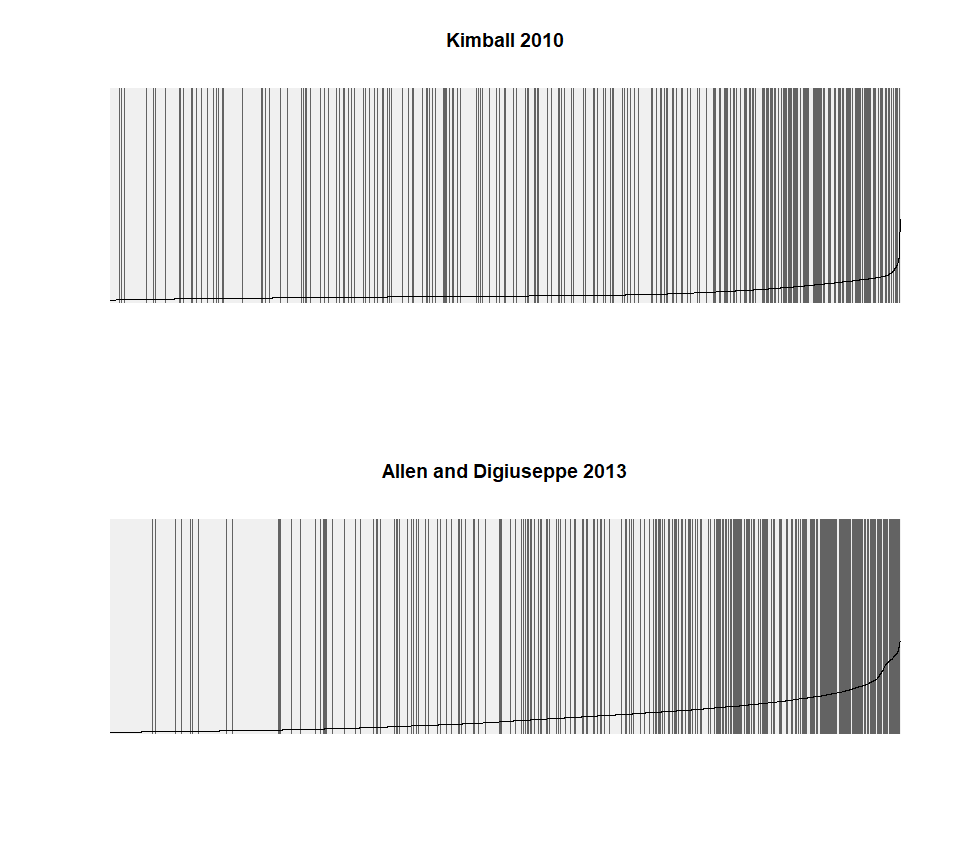
\includegraphics[width=0.90\textwidth]{formation sep_plot.png}
	\caption{Separation plots of primary models from Kimball 2010 and Allen and DiGiuseppe 2013. A separation plot summarizes model fit by ordering observations according to the predicted probability assigned by the model. Dark lines mark observations where the observed value of the dependent variable is one. Better fitting models assign higher predicted probabilities to those observed realizations of the dependent variable, which will be reflected by clustering on the right-hand side of the plot. Greater dispersion of the dark lines indicates that the model does a poor job predicting the outcome of interest.}
	\label{fig:formation sep_plot}
\end{figure}

Besides poor model fit, these two research designs indirectly test the logic of substitution. The key independent variable differentiates between states with high opportunity costs of military spending. But this does not account for differences in national defense burden, or the absolute costs of defense.  
  
Using panel data with a binary indicator of whether a state formed an alliance in a particular year ignores heterogeneity among alliances. Alliances make different promises, and provide different amounts of capability to support those promises. A defense pact with the United States provides more security than a neutrality pact with Senegal, for instance. The choice of alliance types and partners is neglected by these theories and research designs.  


\subsection*{Overall Empirical Assessment}

Although theoretical progress depends on the accumulation of evidence, we have little reliable evidence from 27 studies. What we know about the arms-alliance tradeoff depends on a few studies. Other research designs are narrow, flawed, or both.  

Many of the research design problems in past studies are the result of a levels of analysis problem. There are two distinct levels of analysis in the arms-alliances tradeoff, because international organizations such as alliances are separate from states \citep{Mattes2012, Chibaetal2015}. This difference creates serious measurement problems. 

Measurement of alliance membership is inconsistent across studies. In studies of alliance membership and military spending, scholars have relied on crude summaries of the overall alliance portfolio, or only estimated the impact of a few alliances. Some scholars use a dummy indicator of whether a state has at least one alliance, while others use allied expenditures or capability. Most studies of specific alliances use allied capabilities or expenditures, while general studies use dummy variables. 

State-level dummy indicators of alliance membership are the most common independent variable, but this measure can create a mismatch between the theory and empirical test. For instance, \citet{DigiuseppePoast2016} emphasize differences in alliances, but then examines differences between states. The binary independent variable captures the presence of a defense pact with a democracy, and coupled with a control for defense pacts with non-democracies, they compare states that have a defense pact with a democracy to states with no defense pacts. Their main regression coefficient does not compare alliances, as the theory would lead you to expect. 

Because they average out between-alliance variation, state-level dummies also remove critical details. For instance, democracies tend to form more limited alliance commitments \citep{Chibaetal2015}, so democratic membership and conditionality are correlated. Other factors such as superpower membership, institutionalization, military aid are also correlated with key alliance conditions. Currently, these alliance characteristics are omitted variables, which could affect our estimates of how alliance membership affects military spending. 

Empirical work on the arms-alliances tradeoff faces similar challenges to research on the consequences of membership in international organizations. Selection bias is a ubiquitous concern in that literature \citep{Chaudoinetal2016}, but is not acknowledged in past research designs. And while theory recognizes possible simultaneity between arms and alliances, only one paper (\citep{DigiuseppePoast2016}) uses a simultaneous model. As with theories of the arms-allies tradeoff, there is ample need for improvement in research design.






\section*{Conclusion}

What can we conclude about our understanding of the arms-alliances tradeoff? Despite substantial attention to this question, we know surprisingly little about the connection between alliance behavior and military spending. Substitution and complementarity theories provide some useful insights, but most research designs suffer from serious shortcomings. As a result, there is ample room for theoretical and empirical progress in this literature. 

Progress will require less emphasis on free-riding. While free-riding is a useful rhetorical and analytic device, its applicability to alliances is uncertain at best. Distinguishing between exchange among alliance partners and free riding is difficult theoretically and empirically. Scholars would be better served by considering how alliance membership affects defense spending, without the distraction of trying to identify models of relative defense burdens. Given the policy salience of free-riding claims, scholars should not ignore this concept, but it creates more problems than it solves for scholarship on the arms-alliances tradeoff. 

To improve our understanding of the arms-alliances tradeoff, scholars should improve existing theory and research design in work on how alliance membership affects military spending, and then consider novel research questions. To start, theory must move past the complements-substitutes debate.  


\subsection*{Theory} 

The relationship between arms and alliances is probably conditional--- arms and alliances are not uniformly complements or substitutes. The best research design finds only credible alliances are a substitute for domestic arms, which suggests that a conditional explanation is plausible. Scholars can use components from complementarity and substitution theories identify when alliance membership decreases or increases spending. This endeavor should incorporate domestic incentives to reduce military spending and diverse foreign policy goals, and can build on a shared aspect of the two theories. 

Complementarity and substitution theories use an income effect to connect alliances with changes in military spending. Income effects address how an actor changes the mix of goods it consumes after an increase in its budget. Both paradigms expect the capability gains from an alliance to lead to consumption changes, the difference is that they focus on changes in of different goods. Substitution theory emphasizes shifts in domestic consumption, while complementarity theories consider changes in foreign policy. 

To identify when arms and allies are complements or substitutes, the key task is articulating when states emphasize domestic or international gains. Alliance treaty design may reflect the focus of their members. Alliances can produce security or autonomy for members, which are distinct purposes \citep{Morrow1991}. Security reflects interests in maintaining the international status quo, while autonomy is the ability of states to seek change. Security-producing alliances will facilitate domestic gains, while autonomy-generating alliances will lead to foreign policy gains. If not the security-autonomy distinction, alliance heterogeneity will play an important role in theory. 

In addition to differences between alliances, scholars should address changes in the nature of military spending. The price and complexity of conventional weapons has increased over time, especially in the 20th century \citep{Bitzinger2003}. The marginal capability purchased by a dollar of military spending is decreasing, which affects the purchasing power of small states, and may alter their mix of security policies. And as the time needed to build of complex weapons systems increases, domestic arms will become a more imperfect substitute for alliances, because capability gains from arms investment will take longer to realize. 

Last, theory must provide better guidance for research design. Clear scope conditions are indispensable. If smaller states are more likely to use alliances as a source of security, rather than to increase their foreign policy autonomy \citep{Morrow1991}, then autonomy-seeking major powers have less incentive to substitute alliances for arms. Other theories beyond the economic theory of alliances must consider these and other differences between major and minor powers. 

Besides articulating scope conditions, theory must clarify whether alliance membership or capability impacts domestic arms. It is reasonable to expect that more capable alliances are more valuable to their members. So the capability an alliance brings is a key source of alliance heterogeneity, and research design should reflect this.

\subsection*{Research Design} 

Future research designs should connect to the implications of new theory developments, and chart a middle course between the specific and general studies in previous work. General studies of how the association between alliance behavior and military spending covered a wide universe of cases, but ignored alliance heterogeneity. Studies of specific alliances sacrificed generality for detailed examination of particular treaties. 

The gap between specific and general studies reflects difficulties from moving between different levels of analysis. \citep{Chaudoinetal2015} provide a theoretical and empirical framework of how scholars can consider the role of different levels of analysis in international relations. While they focus on the association between systemic and domestic factors, their approach can be extended to cover membership in international institutions like alliances. 

Multilevel models can compromise between the specific and general approaches by incorporating the alliance and state levels of analysis. Modeling variation at the alliance and state levels will allow for more detailed comparisons of states and alliances. These comparisons are essential for testing any conditional theories that ascribe differences in the arms-alliances tradeoff to different alliance characteristics. 

For modeling how the cost of arms affect alliance formation, it is unclear whether the panel data research designs of \citet{Kimball2010, AllenDigiuseppe2013} are the best approach. Other approaches to modeling alliance formation, including dyadic, k-adic, or network analysis, could capture strategic elements of alliance formation, which are otherwise omitted. But the panel design can be incorporated into a simultaneous model with alliance formation. 

Simultaneity and selection bias are critical issues, but there are several possible solutions. In single-equation models, theory can provide guidance about observable correlates of selection that would otherwise generate omitted variable bias. Scholars could also check for selection on unobservables in these models \citep{Chaudoinetal2016}. Simultaneous models of arms and alliances may address selection bias by modeling the alliance formation process and the correlation between the two policies. Even as work to improve research design continues, scholars should examine other open research questions. 


\subsection*{Open Research Questions} 

Some open research questions are simple empirical tests of other predictions from substitution and complementarity theories, besides the association between alliance membership and military spending. Testing these other predictions will provide additional evidence about the accuracy of these theories. For instance, we know very little about how the cost of domestic arms affects alliance formation, though substitution theory expects a positive relationship between these variables. This test will need a direct measure the costs of defense. The defense burden or the costs of leading weapons systems are two possible measures. 

Other research questions are more novel. Do changes in the rate of alliance fulfillment over time affect domestic military spending? Do other characteristics of an alliance besides democratic membership affect its credibility? What is the role of arms imports for protege states? How does the international context alter the arms-alliances tradeoff? 

Understanding the role of the international context in the arms-alliances tradeoff is especially important. Between nuclear weapons, changing norms about international conquest \citep{Fazal2011}, and economic interdependence \citep{Frieden2006}, the international environment has changed in dramatic ways, especially after 1945. So far, no theories of the arms-alliances tradeoff have addressed whether these shifts in the international environment alter the value of alliances or military spending, and whether context is a control or modifying variable. 

These research questions have tremendous academic and policy importance. The academic rhetoric of free-riding has an outsized impact on popular perceptions of how alliance membership affects defense spending. But the true association may be more nuanced, which should affect our view of the value and purpose of alliances.  

Despite the importance of arms and alliances, there is much we do not know about the relationship between these policies. Improving theory and research design to address how alliance membership affects military spending is the first task. Then scholars can address other open research questions to increase our understanding of the arms-alliances tradeoff.  




%\bibliography{C:/Users/jkalley14/Dropbox/Research/MasterBibliography}  
\bibliography{C:/Users/Josh/Dropbox/Research/MasterBibliography} 





\end{document}